\section{Die Sprache der Mengenlehre}

Die Mengenlehre wurde gegen Ende des 19.\ Jahrhunderts von Georg Cantor (1845--1918) entwickelt, um den Begriff der Unendlichkeit erfassen zu können. Heute ist die Mengenlehre einerseits eine eigenständige mathematische Disziplin, auf der anderen Seite werden die einfachen Grundbegriffe der Mengenlehre in den meisten mathematischen Disziplinen -- und auch außerhalb der Mathematik -- als »Sprache« verwendet, um Gesamtheiten und deren Beziehungen zueinander präzise zu beschreiben. In der vorliegenden Lerneinheit werden nur diese einfachen Grundbegriffe zur Sprache kommen.

\subsection{Beschreibung von Mengen}

Die folgende Formulierung stammt von dem oben erwähnten Georg Cantor selbst:

\begin{quote}
  Unter einer \textbf{Menge} verstehen wir jede Zusammenfassung $M$ von bestimmten wohlunterschiedenen Objekten $m$ unserer Anschauung oder unseres Denken -- welche Elemente der Menge genannt werden -- zu einem Ganzen.
\end{quote}

\subsubsection{Erste Beispiele}

\begin{enumerate}[label=\alph*)]
  \item Die natürlichen Zahlen $1, 2, 3, 4, 5, 6$ bilden eine Menge.
  \item Die Gesamtheit aller natürlichen Zahlen $1, 2, 3, 4, 5, 6, 7, \ldots$ bildet eine Menge.
  \item Die Buchstaben des Namens »Erika« bilden eine Menge.
  \item Die am 1.1.2021 um 0 Uhr lebenden Menschen mit deutscher Staatsbürgerschaft bilden eine Menge.\footnote{Der Abschluss eines Beispiels wird im Folgenden durch das Zeichen $\blacklozenge$ markiert.}\beispielende
\end{enumerate}

Bei sämtlichen der in diesen Beispielen aufgeführten Mengen lässt sich stets entscheiden, ob ein Element zu der betreffenden Menge gehört oder nicht. Beispielsweise gehört die Zahl 2 zu der Menge in a), die Zahl 7 aber nicht. Ebenso gehört Angela Merkel zu der Menge in d), Wladimir Putin dagegen nicht.

An dieser Stelle soll jedoch nicht verschwiegen werden, dass die obige allgemeine Mengendefinition auch ihre Tücken hat. Was ist beispielsweise mit der Menge aller PKWs, die morgen an meinem Haus vorbei fahren werden? Hier kann ich nicht entscheiden (zumindest nicht heute), ob ein Element dazu gehört oder nicht.

Anderes Beispiel: Wir wollen die Menge der am 1.1.2021 existierenden außerirdischen Lebewesen betrachten. Hier wissen wir gar nicht, ob diese Menge überhaupt Elemente enthält.

Zu logischen Komplikationen führt schließlich die Betrachtung der Menge aller Mengen, da diese sich selbst als Element enthalten müsste. Diese Komplikationen bekommt man innermathematisch durch eine \textbf{axiomatische Mengenlehre} in den Griff, auf die wir hier selbstverständlich nicht eingehen.

Von diesen ganzen Tücken wird im Folgenden ganz abgesehen, sondern es wird -- wie in der sogenannten \textbf{naiven Mengenlehre} üblich -- stets von »einfachen« Mengen wie im obigen Beispiel ausgegangen, bei denen klar ist, welche Elemente dazu gehören und welche nicht.

Zwei Anmerkungen sind dazu noch wichtig:
\begin{itemize}
  \item Die Elemente einer Menge müssen voneinander unterscheidbar sein, d.\,h. jedes Element kann auch nur einmal enthalten sein. Folglich enthält die Menge der Buchstaben des Wortes »Muttertag« die Elemente M,u,t,e,r,a,g.
  \item Eine Menge ist durch die in ihr enthaltenen Elemente festgelegt und hat keine weiteren Eigenschaften -- kennt man die Elemente, dann kennt man die Menge. Folglich kann es auch nur \emph{eine} Menge ohne Elemente geben, die man die »leere Menge« nennt.
\end{itemize}

Eine Menge kann man entweder durch die Aufzählung ihrer Elemente beschreiben, die üblicherweise zwischen zwei geschweiften Klammern $\{\ldots\}$ aufgelistet werden, oder aber durch die Angabe einer Eigenschaft, die den Elementen der Menge gemeinsam ist.

\subsubsection{Noch einmal die Beispiele aus 1.1.1.1}

\begin{enumerate}[label=\alph*)]
  \item Hier handelt es sich um die Menge $M = \{1,2,3,4,5,6\}$.
  \item Für die Menge der natürlichen Zahlen verwendet man meist die Bezeichnung $\mathbb{N}$, also ist hier $\mathbb{N} = \{1,2,3,4,5,6,7,\ldots\}$.
  \item Man hat $M = \{E, r, i, k, a\}$.
  \item Hier ist $M = \{x \mid x \text{ ist am } 1.1.2021 \text{ um } 0 \text{ Uhr deutscher Staatsbürger}\}$.\beispielende
\end{enumerate}

Wie am Beispiel d) zu sehen, kann eine Menge dadurch beschrieben werden, dass man innerhalb geschweifter Klammern zunächst ein Element stellvertretend nennt, dann folgt ein senkrechter Strich und dahinter eine eindeutige Beschreibung der Elemente.

Zur Bezeichnung von Mengen werden meist große lateinische Buchstaben $A, B, C, \ldots, M, \ldots$ verwendet, für die Elemente benutzt man häufig kleine lateinische Buchstaben $a, b, c, \ldots, x, \ldots$.

Gehört ein Element $x$ zu einer Menge $X$, so schreibt man abkürzend $x \in X$, falls dies nicht der Fall ist, so benutzt man $x \notin X$.

Die \textbf{leere Menge} wird mit dem Symbol $\emptyset$ bezeichnet, man schreibt auch: $\emptyset = \{\}$.

\subsubsection{Beispiele}

\begin{figure}[h]
  \centering
  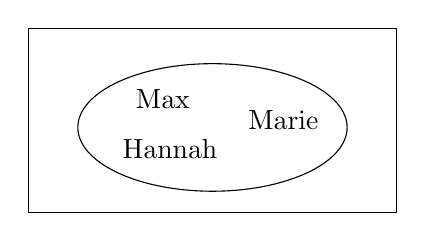
\begin{tikzpicture}[scale=0.9]
    \draw (-2.6,-1.2) rectangle (2.6,1.4);
    \draw (0,0) ellipse (1.9 and 0.9);
    \node at (-0.7,0.4) {Max};
    \node at (1.0,0.1) {Marie};
    \node at (-0.6,-0.3) {Hannah};
  \end{tikzpicture}
  \caption*{Venn-Diagramm der drei Kinder der Familie P.}
\end{figure}

\begin{enumerate}[label=\alph*)]
  \item Hier ist ein Venn-Diagramm der Menge der drei Kinder der Familie P. zu sehen.
  \item Gegeben seien die drei Zahlenmengen $A = \{2,7,11,4\}$, $B = \{3,1500\}$ und $C = \{9\}$. Ein Venn-Diagramm zu den drei Mengen sieht dann so aus.
\end{enumerate}

\begin{figure}[h]
  \centering
  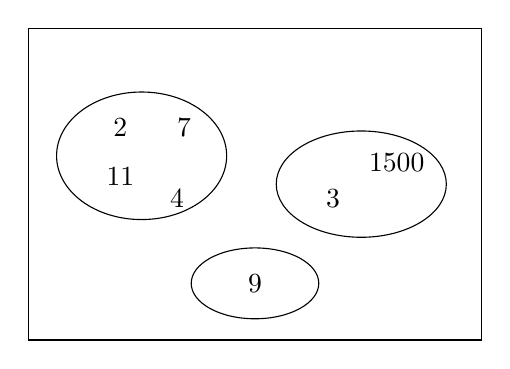
\begin{tikzpicture}[scale=0.9]
    \draw (-3.2,-2.4) rectangle (3.2,2.0);
    \draw (-1.6,0.2) ellipse (1.2 and 0.9);
    \node at (-1.9,0.6) {2}; \node at (-1.0,0.6) {7};
    \node at (-1.9,-0.1) {11}; \node at (-1.1,-0.4) {4};
    \draw (1.5,-0.2) ellipse (1.2 and 0.75);
    \node at (2.0,0.1) {1500}; \node at (1.1,-0.4) {3};
    \draw (0,-1.6) ellipse (0.9 and 0.5);
    \node at (0,-1.6) {9};
  \end{tikzpicture}
  \caption*{Venn-Diagramm zu $A$, $B$ und $C$.}
\end{figure}

\subsection{Beziehungen zwischen Mengen}

Jedes Element der Menge $A=\{2,4\}$ ist auch Element der Menge $B=\{1,2,3,4\}$ -- man sagt, $A$ sei eine Teilmenge von $B$.

\begin{itemize}
  \item Eine Menge $A$ heißt \textbf{Teilmenge} der Menge $B$ (in Symbolen: $A \subseteq B$), wenn jedes Element von $A$ auch Element von $B$ ist.
\end{itemize}

\subsubsection{Beispiele}

\begin{enumerate}[label=\alph*)]
  \item $\{x \mid x \text{ ist Studierende(r) in Hagen}\} \subseteq \{y \mid y \text{ ist Studierende(r) in NRW}\}$\beispielende
  \item Seien $A=\{2,4\}$, $B=\{2,4,6\}$ und $C=\{4,6\}$. Es ist $A\subseteq B$ und $C\subseteq B$. $A\subseteq B$ gilt jedoch beispielsweise nicht, denn das Element 2 aus $A$ gehört nicht zu $C$ -- in einem solchen Fall schreibt man auch $A \not\subseteq C$. Zur Verdeutlichung sind die drei Mengen hier in einem Venn-Diagramm dargestellt:
\end{enumerate}

\begin{figure}[h]
  \centering
  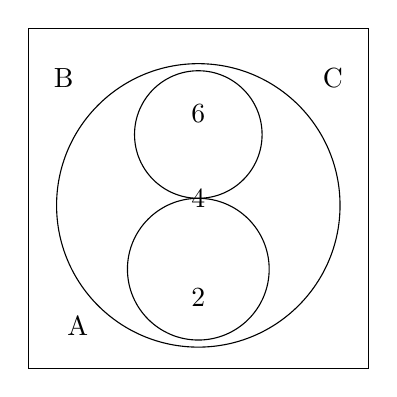
\begin{tikzpicture}[scale=0.9]
    \draw (-2.4,-2.4) rectangle (2.4,2.4);
    \draw (0,-0.1) circle (2.0);
    \draw (0,0.9) circle (0.9) ;
    \draw (0,-1.0) circle (1.0);
    \node at (0,1.2) {6};
    \node at (0,0.0) {4};
    \node at (0,-1.4) {2};
    \node at (-1.9,1.7) {B};
    \node at (1.9,1.7) {C};
    \node at (-1.7,-1.8) {A};
  \end{tikzpicture}
  \caption*{Venn-Diagramm zu $A \subseteq B$ und $C \subseteq B$.}
\end{figure}

Ist sowohl $A\subseteq B$ als auch $B\subseteq A$, so muss $A=B$ sein, da $A$ und $B$ die gleichen Elemente enthalten und eine Menge durch ihre Elemente bestimmt ist.

Ist $A\subseteq B$, jedoch $A\neq B$, so muss es mindestens ein Element von $B$ geben, das nicht zu $A$ gehört -- man sagt hier auch, $A$ sei in $B$ \emph{echt} enthalten und schreibt $A\subset B$ (analog zu $\leq$ und $<$ bei Zahlen).

Die leere Menge ist Teilmenge jeder Menge $M$ ($\emptyset\subseteq M$), auch die Menge $M$ selbst ($M\subseteq M$). Die Menge aller Teilmengen einer Menge $M$ bezeichnet man als \textbf{Potenzmenge} von $M$, in Zeichen: $\mathcal{P}(M)$.

\subsubsection{Beispiel}

Die Menge $A=\{1,2\}$ hat die Potenzmenge $\mathcal{P}(A)=\{\emptyset,\{1\},\{2\},A\}$. Insbesondere gilt also $A\in\mathcal{P}(A)$.\beispielende

\subsection{Mengenoperationen}

Aus vorgegebenen Mengen können weitere Mengen konstruiert werden.

\begin{itemize}
  \item Der \textbf{Durchschnitt} (auch: \textbf{Schnittmenge}) zweier Mengen $A$ und $B$ besteht aus denjenigen Elementen, die sowohl zu $A$ als auch zu $B$ gehören.\\
  Man schreibt: $A\cap B = \{x \mid x\in A \text{ und } x\in B\}$
  \item Die \textbf{Vereinigung} oder \textbf{Vereinigungsmenge} zweier Mengen $A$ und $B$ ist die Menge aller Elemente, die zu mindestens einer der beiden Mengen $A$ oder $B$ gehören.\\
  Man schreibt: $A\cup B = \{x \mid x\in A \text{ oder } x\in B\}$
\end{itemize}

\subsubsection{Beispiel}

Die Mengen $A=\{1,4,6,8\}$ und $B=\{1,6,7\}$ seien vorgegeben. Dann ist $A\cap B=\{1,6\}$ und $A\cup B=\{1,4,6,7,8\}$. Ein Venn-Diagramm sieht so aus:

\begin{figure}[h]
  \centering
  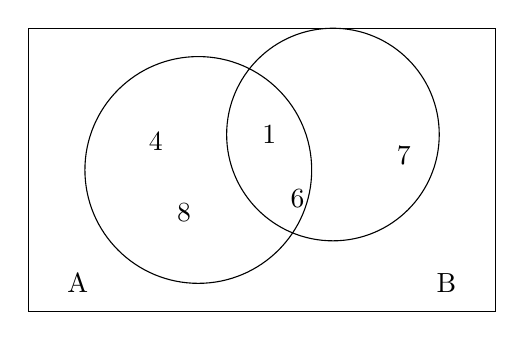
\begin{tikzpicture}[scale=0.9]
    \draw (-3.3,-2.0) rectangle (3.3,2.0);
    \draw (-0.9,0) circle (1.6);
    \draw (1.0,0.5) circle (1.5);
    \node at (-1.5,0.4) {4};
    \node at (-1.1,-0.6) {8};
    \node at (0.1,0.5) {1};
    \node at (0.5,-0.4) {6};
    \node at (2.0,0.2) {7};
    \node at (-2.6,-1.6) {A};
    \node at (2.6,-1.6) {B};
  \end{tikzpicture}
  \caption*{Venn-Diagramm zu $A$ und $B$.}
\end{figure}

\subsubsection{Beispiel}

Sei $K$ die Menge aller Katzen und $S$ die Menge aller schwarzen Tiere. Dann enthält $K \cap S$ alle schwarzen Katzen.
In $K \cup S$ sind alle Tiere, die schwarz oder eine Katze sind, also z.\,B. schwarze Amseln, weiße Katzen, aber auch alle schwarzen Katzen! Graue Elefanten gehören jedoch nicht dazu.\beispielende

\begin{itemize}
  \item Unter der \textbf{Differenz} zweier Mengen $A$ und $B$ versteht man die Menge aller Elemente, die zu $A$, aber nicht zu $B$ gehören.\\
  Man schreibt: $A \setminus B = \{x \mid x\in A \text{ und } x\notin B\}$
\end{itemize}

\subsubsection{Beispiel}

Mit den Mengen $A$ und $B$ aus dem obigen Beispiel 1.1.3.1 ist $A \setminus B = \{4,8\}$ und $B \setminus A = \{7\}$.\beispielende

\begin{itemize}
  \item Es sei $A\subseteq B$. Als \textbf{Komplement} von A bezüglich B wird die Menge aller Elemente bezeichnet, die zu B, aber nicht zu A gehören.\\
  Man schreibt: $\overline{A} = \{x \mid x\in B \text{ und } x\notin A\}$
\end{itemize}

$\overline{A}$ ist hier nichts Anderes als $B\setminus A$ in dem Spezialfall, dass $A\subseteq B$ ist. Um eindeutig auszudrücken, auf welche Obermenge sich das Komplement bezieht, kann man die Obermenge als tiefgestellten Index mit angeben -- man schreibt dann $\overline{A}_B$.

\subsubsection{Beispiel}

Es seien $A = \{2,4\}$, $B = \{2,4,6\}$ und $C = \{2,4,6,8\}$.

Es ist $A \subseteq B \subseteq C$, und für die Komplemente gilt:
$\overline{A}_B = \{6\}$, $\overline{A}_C = \{6,8\}$, $\overline{B}_C = \{8\}$.\beispielende

\subsection{Übungsaufgaben zu Abschnitt 1.1}

\begin{uebungsaufgaben}
  \item Man schreibe die Buchstaben des Wortes »Studium« als Menge.
  \item \begin{enumerate}[label=\alph*)]
      \item Vorgegeben ist die Menge $M = \{1,2,3\}$. Geben Sie alle möglichen Teilmengen von $M$ an.
      \item Wie viele Teilmengen hat die Menge $N = \{1,2,3,4\}$?
      \item Können Sie die Anzahl der Teilmengen der Menge $P = \{1,2,3,4,5,6,7,8,9,10\}$ angeben, ohne alle diese Teilmengen aufzuzählen?\footnote{Es ist keine Schande, wenn man hier nicht auf die richtige Idee kommt.}
    \end{enumerate}
  \item Gegeben seien die folgenden zwei Mengen: $A = \{W, e, r, n, i\}$ und $B = \{x \mid x \text{ ist ein Buchstabe des Namens Werner}\}$. Welche der folgenden Aussagen sind richtig (r) bzw. falsch (f)?
    \begin{enumerate}[label=\alph*)]
      \item $A = B$
      \item $A \subseteq B$
      \item $B \subseteq A$
      \item $i \in A$
      \item $i \in B$
      \item $\{i\} \subseteq A$
    \end{enumerate}
  \item Vorgegeben sind die drei Mengen $A = \{x \in \mathbb{Z} \mid -3 < x < 9\}$, $B = \{2,3,4,5,6,7\}$ und $C = \{y \in \mathbb{Z} \mid y \geq 5\}$. Man bestimme die Mengen $A \cap C$, $A \setminus B$, $\overline{B}_A$, $A \cap \mathbb{N}$, $A \cap (B \cup C)$.
\end{uebungsaufgaben}

\subsection{Lösungen der Übungsaufgaben zu 1.1}

\loesung{1.1.4.1:}
$M = \{S, t, u, d, i, m\}$

\loesung{1.1.4.2:}
\begin{enumerate}[label=\alph*)]
  \item Die acht Teilmengen sind $\emptyset, \{1\}, \{2\}, \{3\}, \{1,2\}, \{1,3\}, \{2,3\}, \{1,2,3\}$.
  \item $N$ besitzt 16 Teilmengen.
  \item $P$ hat $2^{10}$, also 1024 viele Teilmengen.
\end{enumerate}

\loesung{1.1.4.3:}
a) f \qquad b) f \qquad c) r \qquad d) r \qquad e) f \qquad f) r

\loesung{1.1.4.4:}
\begin{align*}
  A \cap C &= \{5,6,7,8\}\\
  A \setminus B &= \{-2,-1,0,1,8\}\\
  \overline{B}_A &= A \setminus B = \{-2,-1,0,1,8\}\\
  A \cap \mathbb{N} &= \{x \in \mathbb{N} \mid 1 \leq x \leq 8\}\\
  A \cap (B \cup C) &= \{x \in \mathbb{Z} \mid 2 \leq x \leq 8\}
\end{align*}
